\section{Pianificazione}
La pianificazione del progetto viene suddivisa nei seguenti periodi:
\begin{itemize}
	\item \textbf{Analisi dei requisiti;}
	\item \textbf{Presentazione RR;}
	\item \textbf{Progettazione architetturale;}
	\item \textbf{Progettazione di dettaglio e codifica;}
	\item \textbf{Validazione e collaudo.}
\end{itemize}
Ogni periodo ha la sua corrispettiva scadenza (vedi 1.5) e la sua implementazione è considerata pronta per la verifica finale e accettazione quando tutte le sotto-attività atomiche sono complete. Vista la scelta di sviluppo seguendo il modello incrementale, per ogni periodo vengono definiti degli incrementi (e relative milestone).
\subsection{Analisi dei requisiti}
\begin{figure}[h!]
	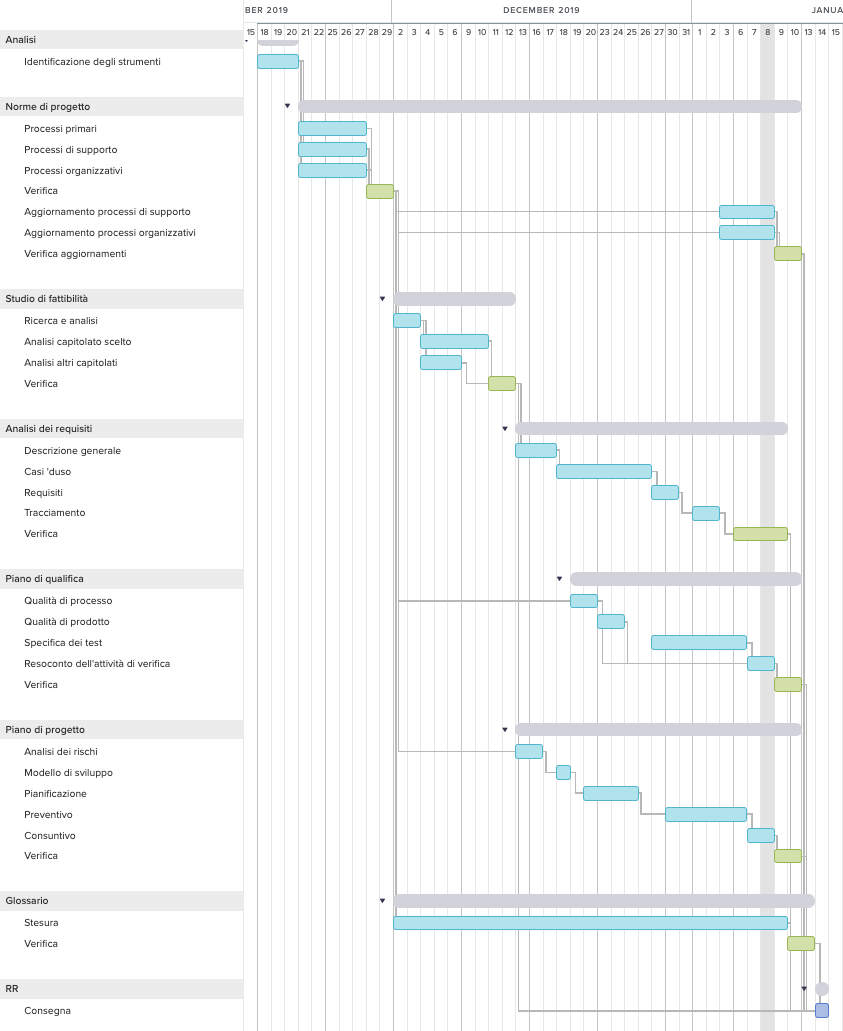
\includegraphics[width=\textwidth]{res/img/g1113}
	\caption{Pianificazione - Analisi dei requisiti}
\end{figure}
Questo periodo è composto dalle seguenti attività:
\begin{itemize}
	\item \textbf{Individuazione degli strumenti:} questa attività consiste nel determinare quali strumenti il gruppo deve utilizzare per la comunicazione, per la stesura dei documenti, per il versionamento, lo sviluppo e la verifica del software;
	\item \textbf{Norme di Progetto:} sono definite tutte le regole utili per lo svolgimento del progetto, relative al prodotto da realizzare e ai processi da adottare. Il documento \textit{Norme di Progetto 1.3.1}\doc viene redatto dall'Amministratore per conto del Responsabile di progetto e viene costantemente aggiornato;
	\item \textbf{Studio di fattibilità:} in questa attività gli analisti effettuano uno studio approfondito dei capitolati in modo da determinare quale di essi verrà scelto. Questa attività è da considerarsi bloccante per l’attività di Analisi dei Requisiti;
	\item \textbf{Analisi dei Requisiti:} durante questa attività vengono identificati ed analizzati i requisiti del capitolato scelto nell'attività di studio di fattibilità e il relativo documento viene composto dagli Analisti;
	\item \textbf{Piano di Qualifica:} in questa attività si individuano le metodologie attraverso le quali si garantisce la qualità del prodotto. A supporto di ciò viene redatto il documento Piano di Qualifica da parte dell'Amministratore e per la parte programmatica dal Progettista;
	\item \textbf{Glossario:} tutti i termini che possono risultare ambigui vengono individuati e definiti nel documento \textit{Glossario 1.0.0}\docs, che viene redatto durante tutta l'analisi dei requisiti.
\end{itemize}
\newpage
\subsection{Presentazione RR}
\begin{figure}[h!]
	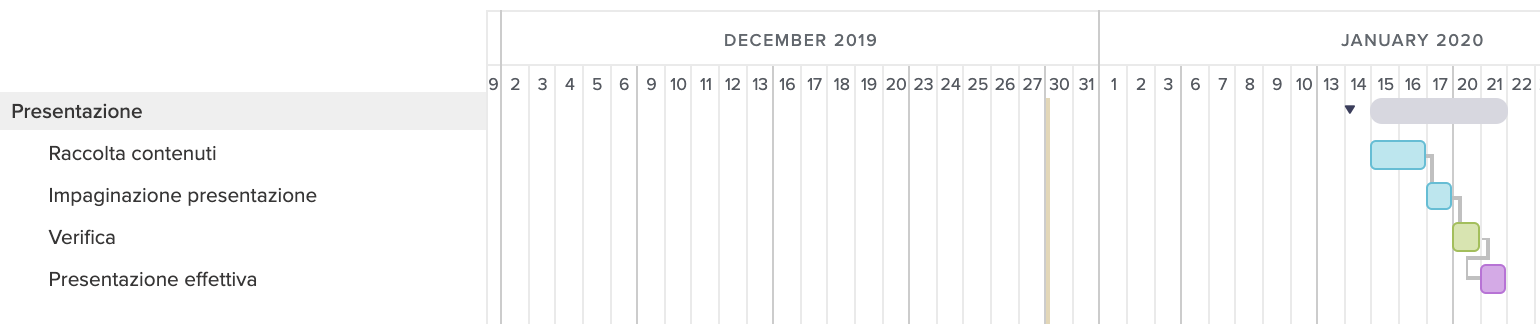
\includegraphics[width=\textwidth]{res/img/g2}
	\caption{Pianificazione presentazione RR}
\end{figure}
Viene fornita una pianificazione per la predisposizione e preparazione dei contenuti per la presentazione alla revisione formale.
\newpage
\subsection{Progettazione architetturale}
Questo periodo ha come obbiettivo l'individualizzazione di una soluzione architetturale che soddisfi i requisiti del prodotto ed è stata suddiviso nelle attività:
\begin{itemize}
	\item \textbf{Technology \textit{Baseline\glos}:} redazione di un documento nel quale vengono individuati e specificati i pattern architetturali utilizzati negli ambiti delle tecnologie coinvolte;
	\item  \textbf{Proof of concept:} codifica di una bozza del prodotto per verificare la correttezza dell'architettura del sistema;
	\item \textbf{Documentazione:} incremento della documentazione in base ai nuovi dati rilevati.
\end{itemize}
\subsubsection{Proof Of Concept}
Sono state identificate tre aree di interesse tecnologico principali:
\begin{itemize}
	\item \textbf{Smart Contract}: contratto Ethereum\glo, fulcro del funzionamento di \textit{Etherless}
	\item \textbf{Comunicazione tra client e server}: applicativo client e server devono scambiarsi dati attraverso lo smart contract
	\item \textbf{Serverless\glo}: ambiente server convertito in ambiente serverless\glo
\end{itemize}
Questi Proof Of Concept saranno la base della costruzione dei componenti finali di \textit{Etherless}, ovvero \textit{eth-smart, eth-client, eth-server}.
\subsubsection{Incrementi e milestone}
\begin{itemize}
	\item \textbf{\RomanNumeralCaps{1} Incremento:} (entro il 19.02.2020) Correzione e integrazione documenti in base alle conoscenze acquisite durante l'Analisi dei requisiti;
	\item \textbf{\RomanNumeralCaps{2} Incremento:} (entro il 25.02.2020) Realizzazione del primo Proof Of Concept (Smart Contract);
	\item \textbf{\RomanNumeralCaps{3} Incremento:} (entro il 28.02.2020) Realizzazione del secondo Proof Of Concept (Comunicazione tra client e server);
	\item \textbf{\RomanNumeralCaps{4} Incremento:} (entro il 05.03.2020) Realizzazione del terzo Proof Of Concept (Serverless);
	\item \textbf{\RomanNumeralCaps{5} Incremento:} (entro il 9.03.2020) Aggiornamento dei documenti;
	\item \textbf{\RomanNumeralCaps{6} Incremento:} (entro il 16.03.2020) Presentazione RP;
\end{itemize}
	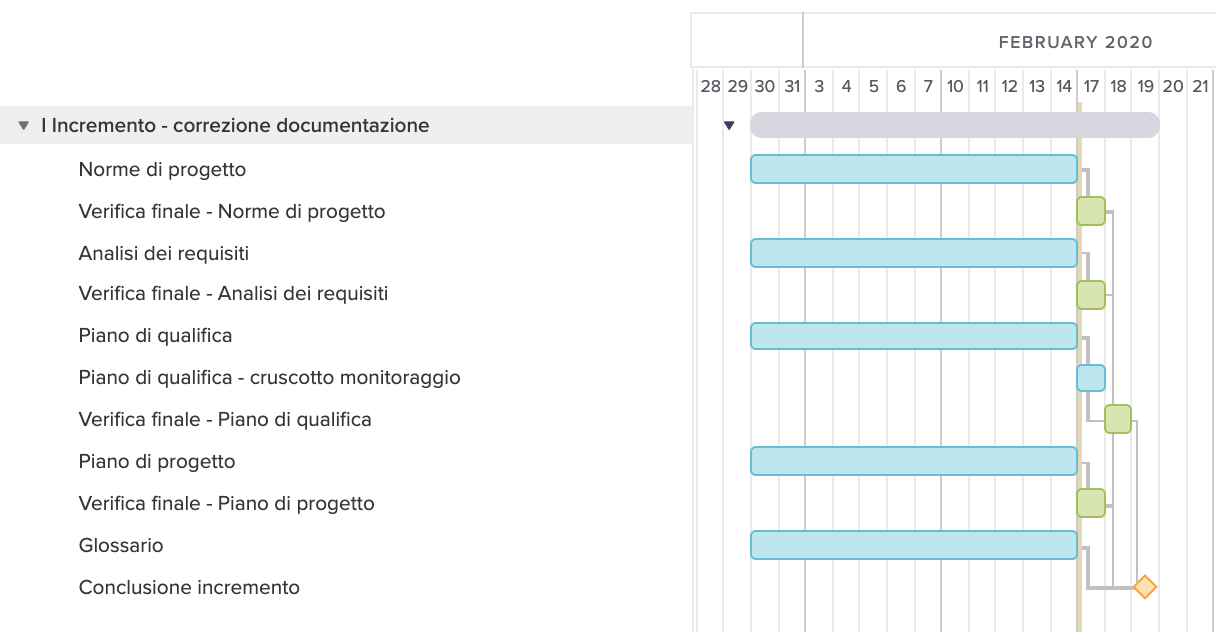
\includegraphics[width=\textwidth]{res/img/gantt/RP/1}
	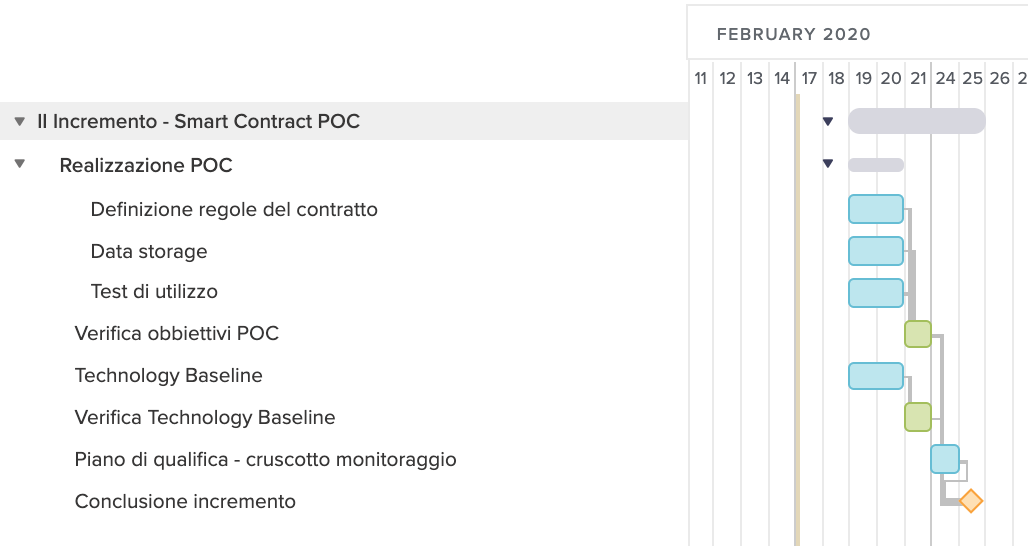
\includegraphics[width=\textwidth]{res/img/gantt/RP/2}
	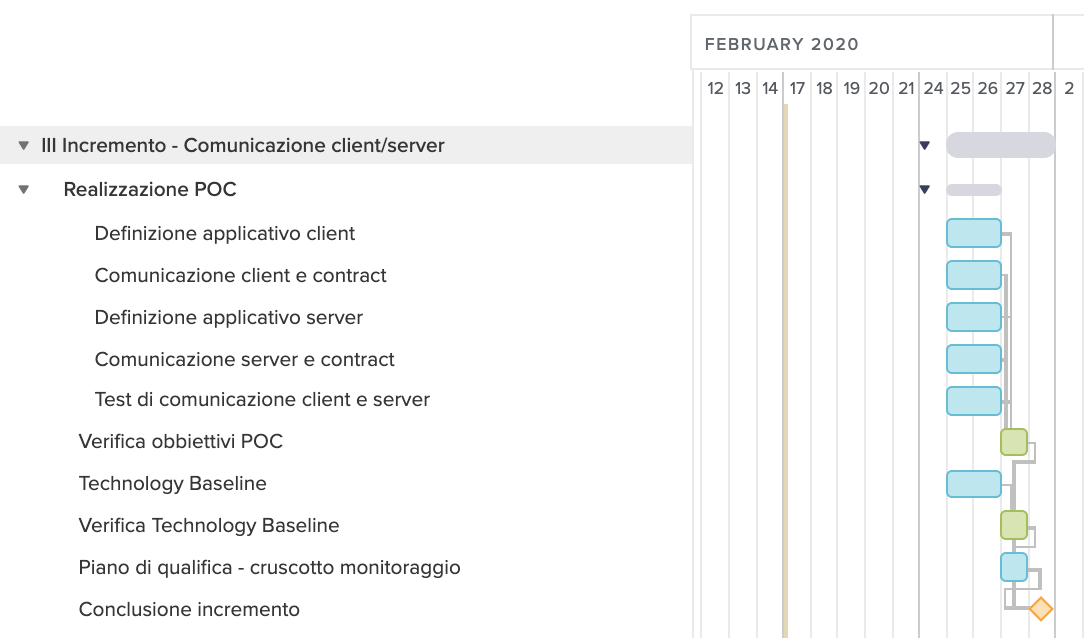
\includegraphics[width=\textwidth]{res/img/gantt/RP/3}
	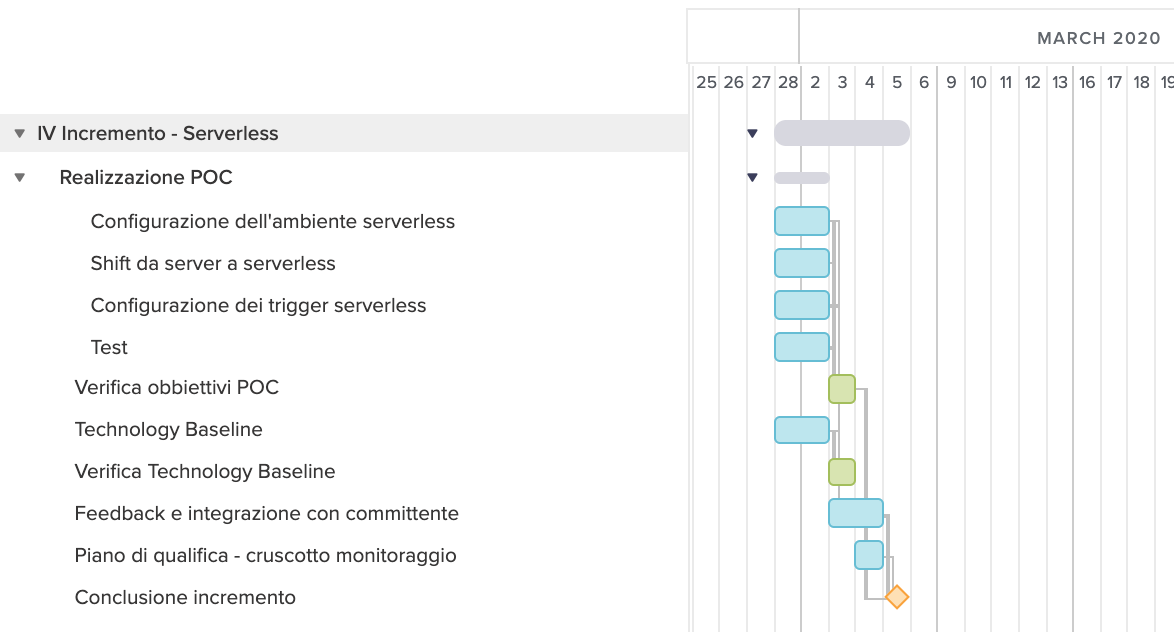
\includegraphics[width=\textwidth]{res/img/gantt/RP/4}
	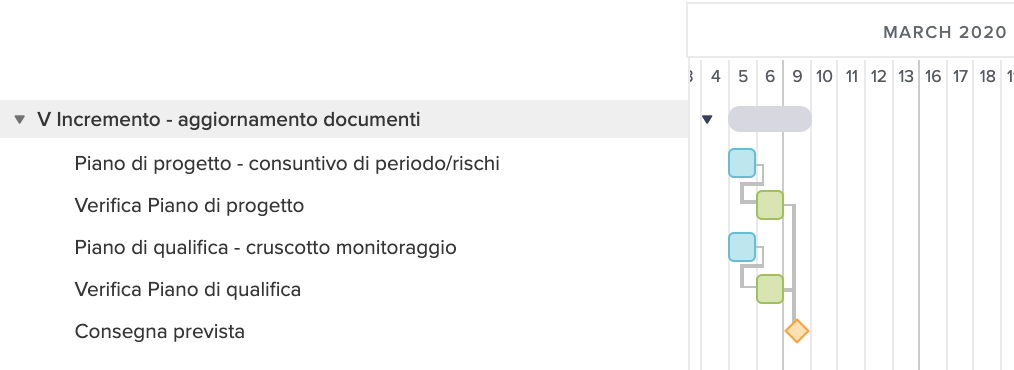
\includegraphics[width=\textwidth]{res/img/gantt/RP/5}
	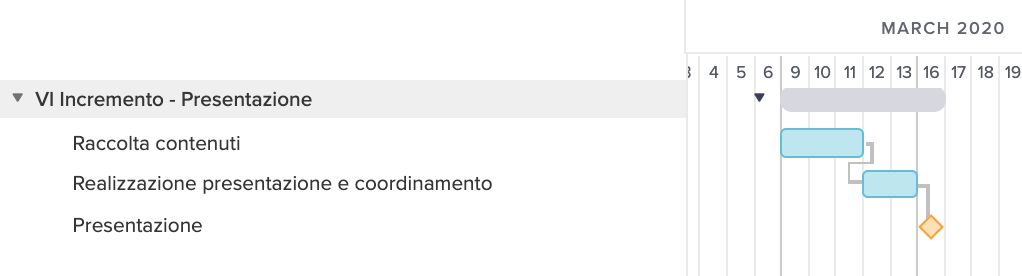
\includegraphics[width=\textwidth]{res/img/gantt/RP/6}
\begin{figure}[h!]
	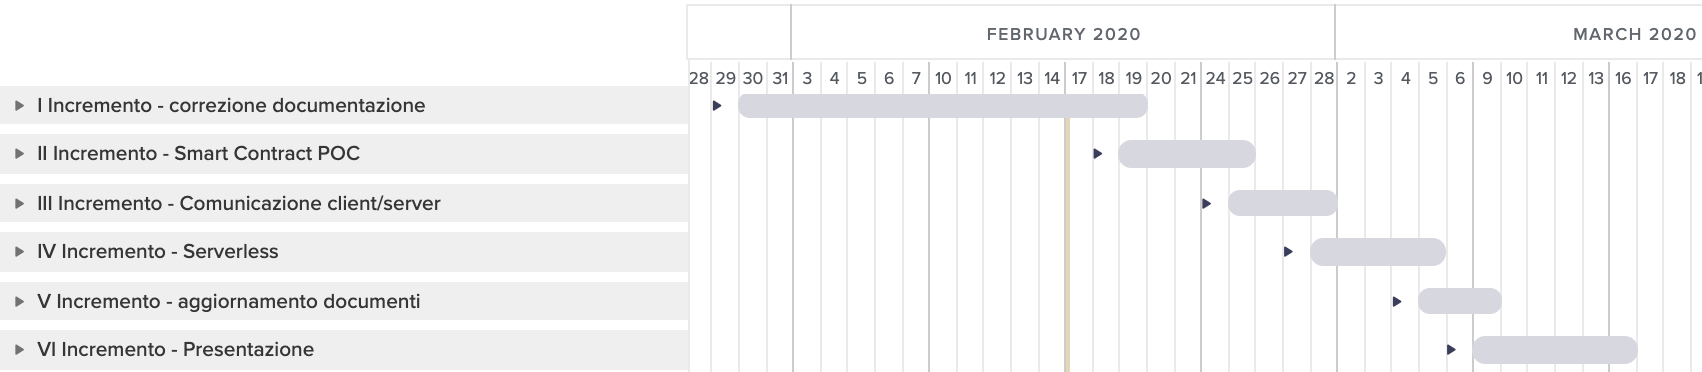
\includegraphics[width=\textwidth]{res/img/gantt/RP/f}
	\caption{Pianificazione Progettazione architetturale}
\end{figure}
\newpage
\subsection{Progettazione di dettaglio e codifica}

\noindent Questo periodo è stata suddiviso nelle attività:
\begin{itemize}
	\item \textbf{Specifiche di prodotto:} documento nel quale vengono individuate le unità che costituiscono il prodotto; viene eseguita una progettazione dettagliata in modo da permettere la successiva codifica delle funzionalità;
	\item  \textbf{Codifica:} implementazione del prodotto;
	\item \textbf{Manuale utente:} realizzazione del \textit{Manuale Utente} per l'utilizzo del prodotto;
	\item \textbf{Documentazione:} incremento della documentazione in base ai nuovi dati rilevati.
\end{itemize}
\subsubsection{Componenti}
Per la realizzazione del prodotto software è necessaria la codifica e la completa conformità di \textit{eth-smart, eth-client, eth-server} ai requisiti del committente e ai casi d'uso.
\subsubsection{Incrementi e milestone}
\begin{itemize}
	\item \textbf{\RomanNumeralCaps{1} Incremento:} (entro il 20.03.2020) Correzione e integrazione documenti in base alle conoscenze acquisite durante la Progettazione architetturale;
	\item \textbf{\RomanNumeralCaps{2} Incremento:} (entro il 27.02.2020) Collaudo ed eventuali correzioni;
	\item \textbf{\RomanNumeralCaps{3} Incremento:} (entro il 03.04.2020) Documentazione codice;
	\item \textbf{\RomanNumeralCaps{4} Incremento:} (entro il 09.04.2020) Test di accettazione e rilascio in ambiente di produzione;
	\item \textbf{\RomanNumeralCaps{5} Incremento:} (entro il 13.04.2020) Aggiornamento documenti e consuntivo finale;
	\item \textbf{\RomanNumeralCaps{5} Incremento:} (entro il 20.03.2020) Presentazione RA;
\end{itemize}
	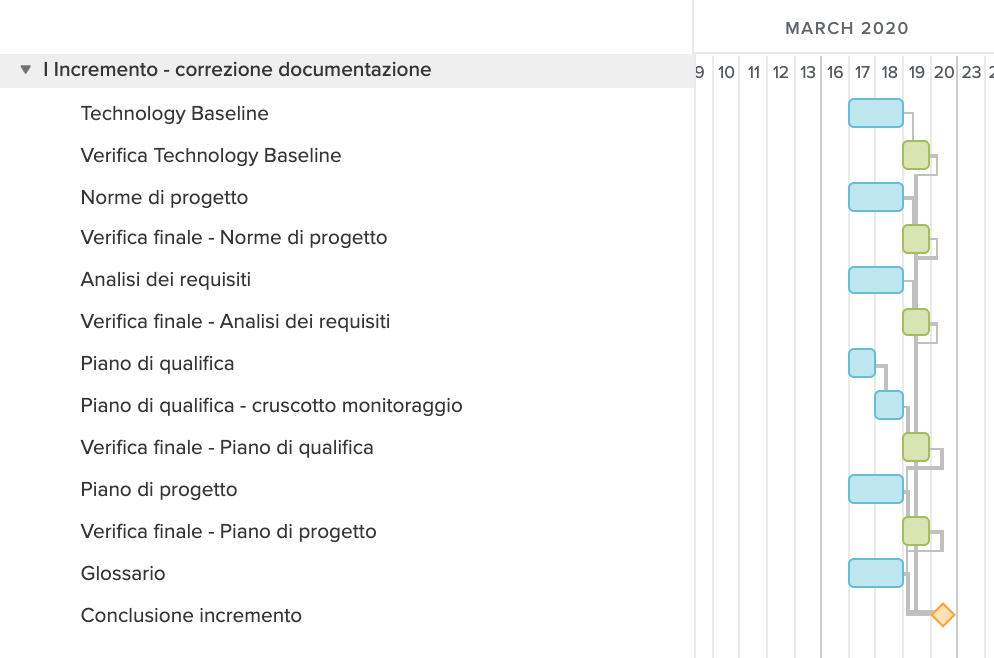
\includegraphics[width=\textwidth]{res/img/gantt/RQ/1}
	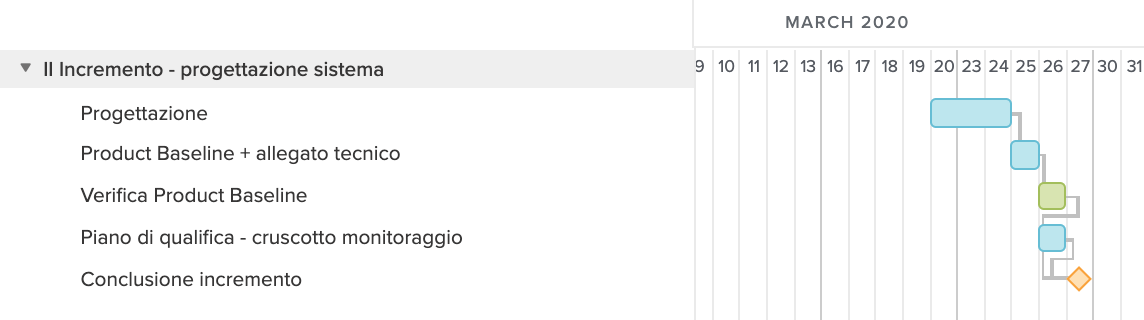
\includegraphics[width=\textwidth]{res/img/gantt/RQ/2}
	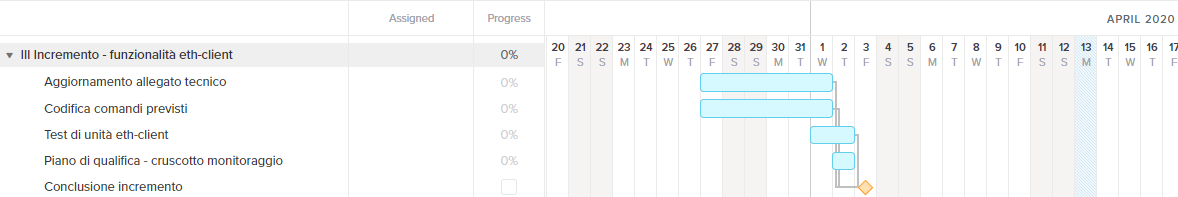
\includegraphics[width=\textwidth]{res/img/gantt/RQ/3}
	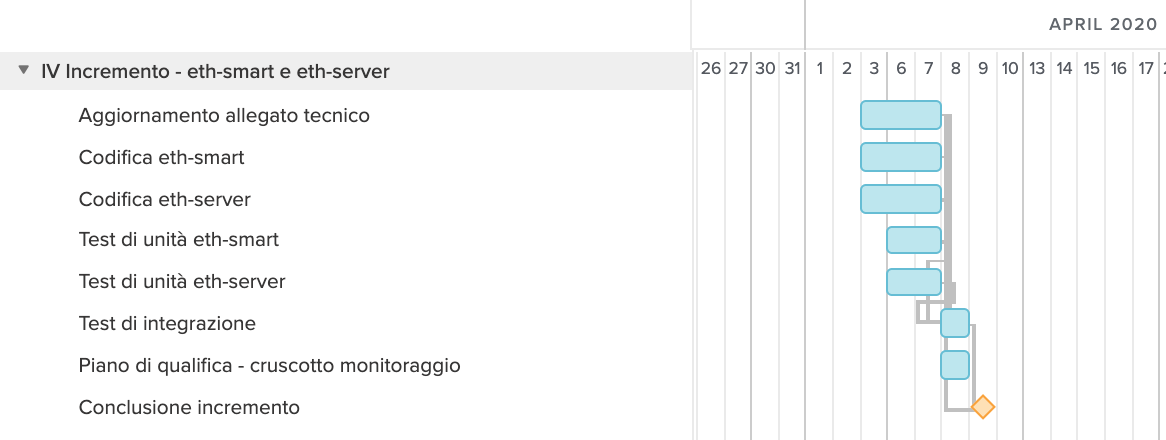
\includegraphics[width=\textwidth]{res/img/gantt/RQ/4}
	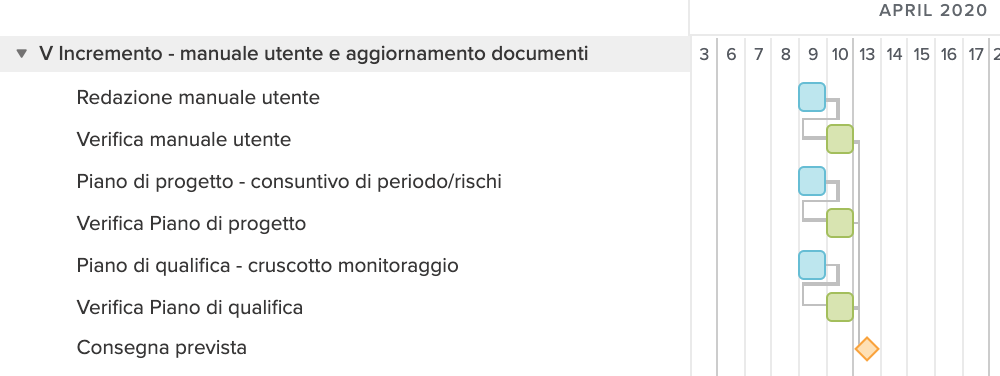
\includegraphics[width=\textwidth]{res/img/gantt/RQ/5}	
	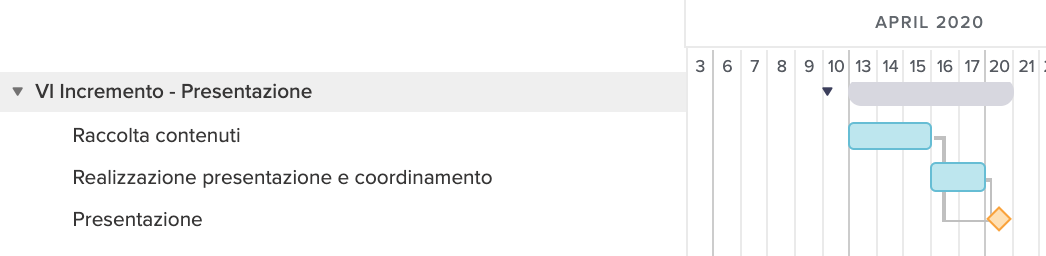
\includegraphics[width=\textwidth]{res/img/gantt/RQ/6}
\begin{figure}[h!]
	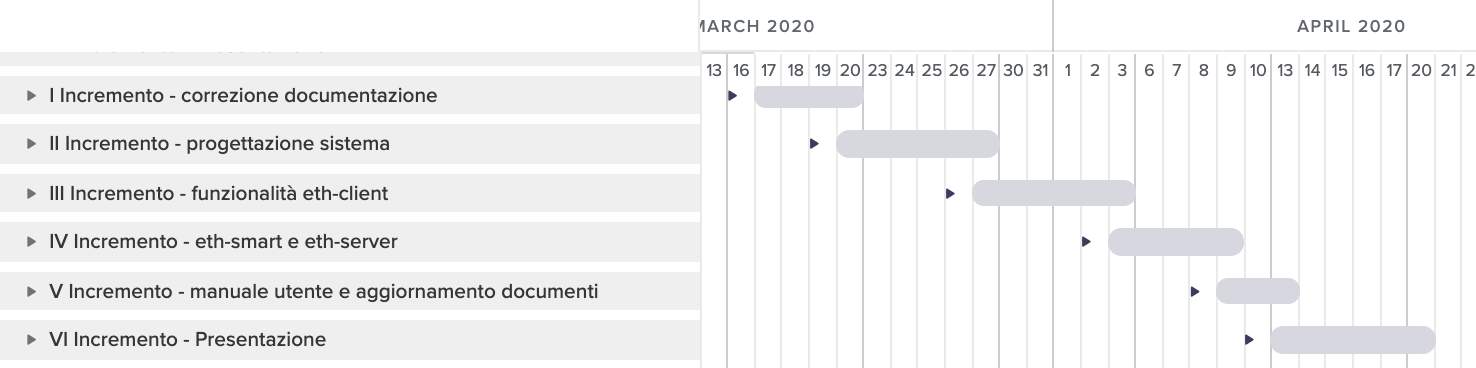
\includegraphics[width=\textwidth]{res/img/gantt/RQ/f}
	\caption{Pianificazione Progettazione di dettaglio}
\end{figure}
\subsection{Validazione e collaudo}
Questo periodo è stati suddiviso nelle attività:
\begin{itemize}
	\item \textbf{Codifica:} modifica del codice se necessario apportare correzioni;
	\item \textbf{Documentazione codice:} realizzazione della documentazione relativa al codice scritto, con lo scopo di fornire informazioni necessarie alla manutenzione del software;
	\item \textbf{Validazione e Collaudo:} controlli per verificare la conformità alle del prodotto ai bisogni del cliente;
	\item \textbf{Documentazione:} incremento della documentazione in base ai nuovi dati rilevati.
\end{itemize}
\subsubsection{Incrementi e milestone}
\begin{itemize}
	\item \textbf{\RomanNumeralCaps{1} Incremento:} (entro il 29.04.2020) Correzione e integrazione documenti in base alle conoscenze acquisite durante la Progettazione di dettaglio e codifica;
	\item \textbf{\RomanNumeralCaps{2} Incremento:} (entro il 04.05.2020) Progettazione di dettaglio e allegato tecnico;
	\item \textbf{\RomanNumeralCaps{3} Incremento:} (entro il 07.04.2020) Sviluppo delle funzionalità di \textit{eth-client};
	\item \textbf{\RomanNumeralCaps{4} Incremento:} (entro il 09.04.2020) Sviluppo completo di \textit{eth-smart} e ottimizzazione di \textit{eth-server}; test di integrazione;
	\item \textbf{\RomanNumeralCaps{5} Incremento:} (entro il 11.04.2020) Manuale utente; aggiornamento dei documenti;
	\item \textbf{\RomanNumeralCaps{5} Incremento:} (entro il 28.03.2020) Presentazione RA;
\end{itemize}
	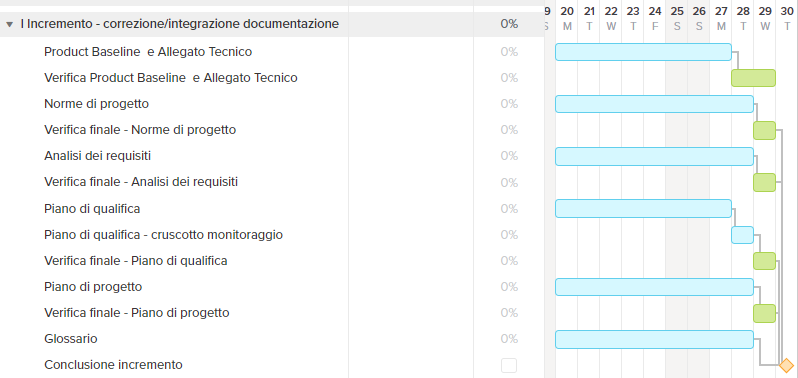
\includegraphics[width=\textwidth]{res/img/gantt/RA/1}
	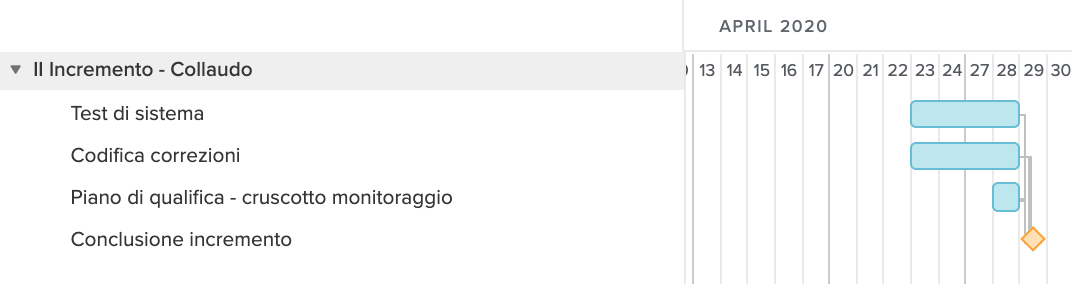
\includegraphics[width=\textwidth]{res/img/gantt/RA/2}
	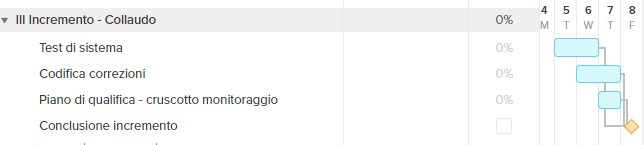
\includegraphics[width=\textwidth]{res/img/gantt/RA/3}
	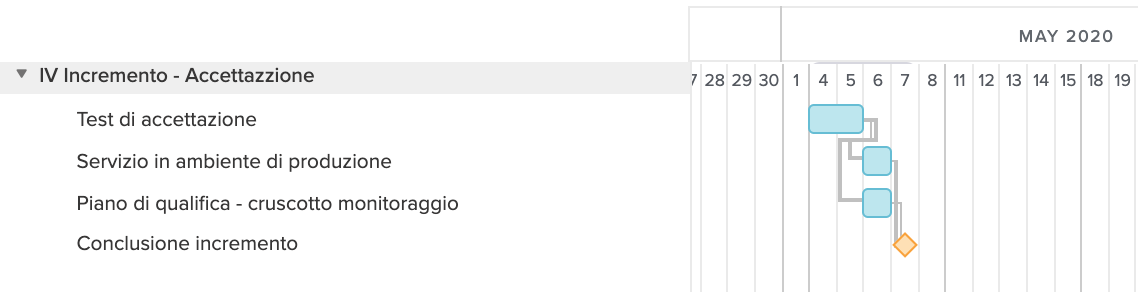
\includegraphics[width=\textwidth]{res/img/gantt/RA/4}
	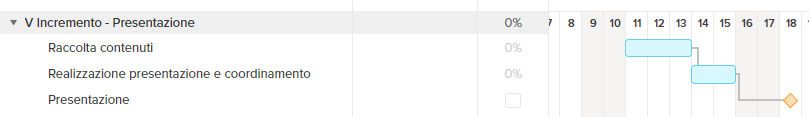
\includegraphics[width=\textwidth]{res/img/gantt/RA/5}
	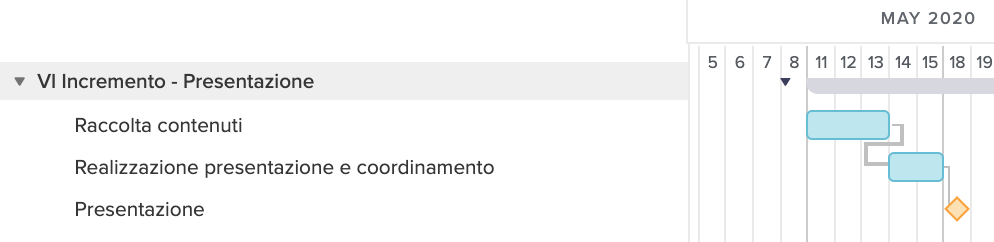
\includegraphics[width=\textwidth]{res/img/gantt/RA/6}
\begin{figure}[h!]
	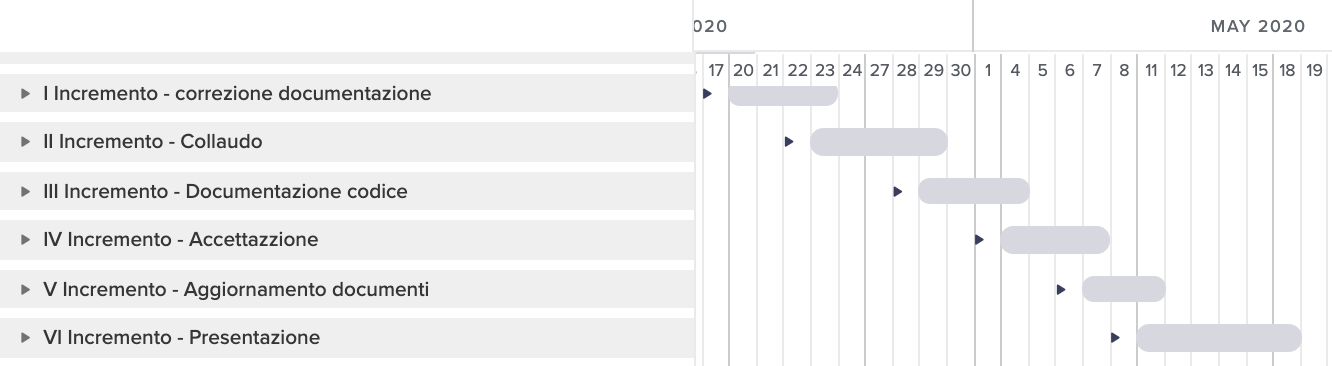
\includegraphics[width=\textwidth]{res/img/gantt/RA/f}
	\caption{Pianificazione Progettazione di dettaglio}
\end{figure}
